\documentclass[runningheads]{llncs}
\usepackage[T1]{fontenc}
\usepackage{hyperref}
\usepackage{xcolor}
\usepackage{booktabs}
%%%%%%%%%%%%%%%%%%%%%%%%%%%%%%%%%%%%%%%%%%%%%%%%%%%%%%%%%%%%
%% Drawing
%%%%%%%%%%%%%%%%%%%%%%%%%%%%%%%%%%%%%%%%%%%%%%%%%%%%%%%%%%%%
\usepackage{tikz}
\usepackage{amsfonts}

\usetikzlibrary{positioning,automata} % drawing automa
\usetikzlibrary{calc,fit,tikzmark}

% for captions in figures
\usepackage{subcaption}

% hyperref for LNCS
\renewcommand\UrlFont{\color{blue}\rmfamily}

\newcommand{\vangiang}[1]{\textcolor{magenta}{#1}}
\newcommand{\sylvain}[1]{\textcolor{teal}{#1}}

\begin{document}

\title{Minimal trap spaces of Logical models are maximal siphons of their Petri net encoding}
\titlerunning{Minimal trap spaces as maximal siphons}
% \title{Scaling-up attractor computation for Boolean models}
% \vangiang{I like the first title :). Since we only conduct experiments on real-world Boolean models of not too large size, it seems to make less sense to use "scaling-up" (this should be for the journal version).}

\author{Van-Giang Trinh\inst{1}\orcidID{0000-0001-6581-998X} \and \\
  Sylvain Soliman\inst{2}\orcidID{0000-0001-5525-7418} \and \\
  Kunihiko Hiraishi\inst{3}\orcidID{0000-0003-1750-1891} \and \\ Belaid Benhamou\inst{1}
  }

\authorrunning{Trinh et al.}

\institute{
  LIS, Aix-Marseille Université, Marseille, France\\
  \email{\{trinh.van-giang, belaid.benhamou\}@lis-lab.fr}
  \and
  Lifeware team, Inria Saclay center, Palaiseau, France\\
  \email{Sylvain.Soliman@inria.fr}
  \and
  School of Information Science, Japan Advanced Institute of Science and Technology, Japan\\
  \email{hira@jaist.ac.jp}
}

\maketitle

\begin{abstract}

  Boolean modelling of gene regulation but also post-transcri\-ptomic models has proven over the years that it can bring powerful analyses and corresponding insight to the many cases where precise biological data is not sufficiently available to build a detailed quantitative model.
  This is even more true for very large models where such data is frequently missing and led to a constant increase in size of logical models \emph{à la} Thomas.
  Besides simulation, the analysis of such models is mostly based on attractor computation, since those correspond roughly to observable biological \emph{phenotypes}. The recent use of trap spaces made a real breakthrough in that field allowing to consider medium-sized models that used to be out of reach.
  However, with the continuing increase in model-size, the state-of-the-art computation of minimal trap spaces based on \emph{prime-implicants} shows its limits as there can be a huge number of implicants.

  In this article we present an alternative method to compute minimal trap spaces, and hence complex attractors, of a Boolean model. It replaces the need for prime-implicants by a completely different technique, namely the enumeration of maximal siphons in the Petri net encoding of the original model.
  After some technical preliminaries, we expose the concrete need for such a method and detail its implementation using Answer Set Programming.
  We then demonstrate its efficiency and compare it to implicant-based methods on some large Boolean models from the literature.

\keywords{Logical models \and Boolean models \and Trap spaces \and Attractor computation \and Petri nets \and Siphons}
\end{abstract}

\section{Introduction}

From the observation that the transcriptional regulation behaved in a sigmoid step-like way, came the original idea to represent models of gene regulation as discrete event systems.
Those Gene Regulation Networks (GRN) use thresholds or equivalently logical functions to represent the different regulations~\cite{glass1973logical,thomas1973boolean,thomas1990biological,thomas1991regulatory}.

Boolean modelling has proven over the years that it can bring powerful analyses and corresponding insight to the many cases where precise biological data is not sufficiently available to build a detailed quantitative model~\cite{wang2012boolean}, even for modelling post-transcriptional mechanisms.
This is even more true for very large models where such data is frequently missing and led to a constant increase in size of logical models \emph{à la} Thomas~\cite{aghamiri2020automated}.
Besides simulation, the analysis of such models is mostly based on attractor computation, since those correspond roughly to observable biological \emph{phenotypes}. The recent use of trap spaces~\cite{klarner2015computing} made a real breakthrough in that field allowing to consider medium-sized models that used to be out of reach.
However, with the continuing increase in model-size, the state of the art computation of minimal trap spaces based on \emph{prime-implicants} shows its limits as there can be a huge number of implicants.

Petri nets were introduced in the 60’s as a simple formalism for describing and analyzing information processing systems that are characterized as being concurrent, asynchronous, non-deterministic and possibly distributed~\cite{peterson1981petri,Murata1989}.
The use of Petri nets for representing biochemical reaction systems, by mapping molecular species to places and reactions to transitions, was introduced quite late in~\cite{reddy1993petri}, together with some Petri net concepts and tools for the analysis of metabolic networks.
Siphons are such a concept but they have not been used a lot for the analysis of biochemical systems even if the practical cost of computing their minimal/maximal elements appear much more manageable than the theoretical complexity would indicate~\cite{nabli2016enumerating}.

In this article we present an alternative method to compute minimal trap spaces, and hence complex attractors, of a Boolean model. It replaces the need for prime-implicants by a completely different technique, namely the enumeration of maximal siphons in the Petri net encoding of the original model.
After some technical preliminaries, we expose the concrete need for such a method and detail its implementation using Answer Set Programming (ASP).
We then demonstrate its efficiency and compare it to implicant-based methods on some large Boolean models from the literature.

All models used for evaluation and the implementation of the presented method are available at\dots.

\sylvain{TBD}

\section{Preliminaries}

We will briefly recall here some preliminaries on Boolean models related to trap spaces and Petri nets.
In the case of multi-level Logical models, an encoding into a Boolean model is always possible~\cite{Didier2011}.

\subsection{Traps spaces}

We recall here some definitions from~\cite{klarner2015computing} for the introduction of \emph{trap spaces}.
Minimal trap spaces prove to be a very good approximation of the attractors of a Boolean model under asynchronous update schemes and have become the \emph{de facto} standard way to analyze models of a few tens of \emph{genes}~\cite{klarner2017pyboolnet,cifuentes2020control}.

%%% Boolean model %%%
Given a Boolean model \(\mathcal{M} = (V, F)\) with variables \(V=(v_{1},\dots,v_{n})\) and Boolean functions \(F=(f_{1},\dots,f_{n})\), its state-space is \(\mathcal{S}_{\mathcal{M}} =\mathbb{B}^{n}\) with \(\mathbb{B} = \{0, 1\}\). A state \(s \in \mathbb{B}^{n}\) is a mapping \(s : V \mapsto \mathbb{B}\) that assigns either 0 (inactive) or 1 (active) to each node. At each time step \(t\), node \(x_i\) can update its state by
\[x_i(t + 1) = f_i(x(t)).\] An update scheme of a Boolean model specifies the way that the nodes of the model update their states through time evolution~\cite{thomas1991regulatory}. There are two main types of update schemes: synchronous and asynchronous.

%%% Trap set %%%
A non-empty set \(T \subseteq S_{\mathcal{M}}\) is a \emph{trap set} of \(\mathcal{M}\) if and only if for every \(x \in T\) and \(y \in S_{\mathcal{M}}\) with \(y\) is reachable from \(x\) it holds that \(y \in T\).

%%% Subspace %%%
A \emph{subspace} \(m\) of \(\mathcal{S}_{\mathcal{M}}\) is characterized by its fixed nodes (denoted by \(D_m\)) and free nodes.
This subspace can be specified by an assignment \(D_m \mapsto \mathbb{B}\) where \(D_m \subseteq V\) and \(m(u)\) is the value of node \(u \in D_m\).
The remaining nodes of \(\mathcal{M}\), \(V \setminus D_m\), are said to be \emph{free}, i.e., they can receive any Boolean value.
We write subspaces like states but use in addition the symbol \(\star\) to indicate that a node is free.
A subspace \(m\) thus corresponds to the set of states \(\mathcal{S}_{\mathcal{M}}[m] := \{s \in \mathcal{S}_{\mathcal{M}}\;|\;\forall x_i \in D_m : s_i = m(x_i)\}\).
For example, \(m = \star\star1\) means that \(D_m = \{x_3\}\), \(m(x_3) = 1\), and corresponds to the set of states \(\{001, 011, 101, 111\}\).
Let \(\mathcal{S}_{\mathcal{M}}^{\star}\) denote the set of all possible subspaces of \(\mathcal{M}\). Note that \(\left|\mathcal{S}_{\mathcal{M}}^{\star}\right| = 3^n\) and \(S_{\mathcal{M}} \subset \mathcal{S}_{\mathcal{M}}^{\star}\)~\cite{klarner2015computing}.

%%% Minimal trap space and example %%%
A \emph{trap space} is defined as a subspace that is also a trap set.
It is noted that trap spaces of a Boolean model are independent of the update scheme of this model~\cite{klarner2015computing}.
Then, we define a partial order \(<\) on \(\mathcal{S}_{\mathcal{M}}^{\star}\) as: \(m < m'\) if and only if \(\mathcal{S}_{\mathcal{M}}[m] \subseteq \mathcal{S}_{\mathcal{M}}[m']\) and \(\mathcal{S}_{\mathcal{M}}[m] \neq \mathcal{S}_{\mathcal{M}}[m']\).
Consequently, a trap space \(m\) is minimal if and only if there is no trap space \(m' \in \mathcal{S}_{\mathcal{M}}^{\star}\) such that \(m' < m\).

%%% Example %%%
For example, let us consider the Boolean model shown in Example~\ref{example:BN}.
Figure~\ref{fig:stg_and_PN}(a) shows the dynamics of this model under the fully asynchronous update (i.e., only one node is nondeterministically selected in order to be updated at each time step).
The model has all two trap spaces, \(m_1 = 11\) and \(m_2 = \star\star\).
Since \(m_1 < m_2\), \(m_1\) is a minimal trap space of the Boolean model.

\begin{example}
We give a Boolean model \(\mathcal{M} = (V, F)\), where \(V = (x_1, x_2)\) and \(F = (f_1, f_2)\) with \(f_1 = (x_1 \land x_2) \lor (\neg x_1 \land \neg x_2), f_2 = (x_1 \land x_2) \lor (\neg x_1 \land \neg x_2)\). Herein, \(\land\), \(\lor\), and \(\neg\) denote the CONJUNCTION, DISJUNCTION, and NEGATION logical operators, respectively.
\label{example:BN}
\end{example}

\begin{figure}[!ht]
\centering
\begin{subfigure}[b]{0.4\textwidth}
\centering
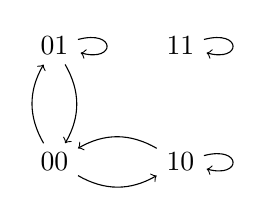
\begin{tikzpicture}[node distance=1cm and 1cm, every node/.style={scale=1.0}]
   \node[] (0) [] {00};
   \node[] (1) [above=of 0] {01};
   \node[] (2) [right=of 0] {10};
   \node[] (3) [above=of 2] {11};
   
   \draw[->] (0) edge [bend left] (1);
   \draw[->] (0) edge [bend right] (2);
   
   \draw[->] (1) edge [bend left] (0);
   \draw[->] (1) edge [loop right] (1);
   
   \draw[->] (2) edge [bend right] (0);
   \draw[->] (2) edge [loop right] (2);
   
   \draw[->] (3) edge [loop right] (3);
\end{tikzpicture}
\caption{}
\end{subfigure}%
\begin{subfigure}[b]{0.6\textwidth}
\centering
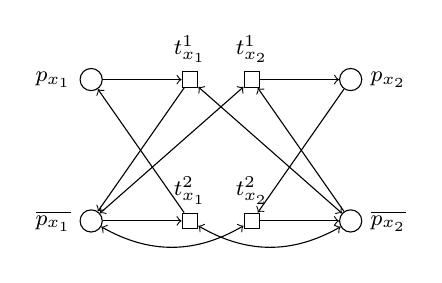
\begin{tikzpicture}[node distance=1cm and 1cm, every node/.style={scale=1.0}]\footnotesize
  \node[circle,draw,label=left:$p_{x_1}$] (x1) {};
  \node[circle,draw,label=left:$\overline{p_{x_1}}$] (nx1) [below=of x1, yshift=-0.5cm] {};
    
  \node[circle,draw,label=right:$p_{x_2}$] (x2) [right=of x1, xshift=2.0cm] {};
  \node[circle,draw,label=right:$\overline{p_{x_2}}$] (nx2) [below=of x2, yshift=-0.5cm] {};
    
  \node[rectangle,draw,label=above:$t^1_{x_1}$] (t1x1) [right=of x1] {};
  \node[rectangle,draw,label=above:$t^2_{x_1}$] (t2x1) [right=of nx1] {};
  
  \node[rectangle,draw,label=above:$t^1_{x_2}$] (t1x2) [left=of x2] {};
  \node[rectangle,draw,label=above:$t^2_{x_2}$] (t2x2) [left=of nx2] {};
  
  \draw[->] (x1) -- (t1x1);
  \draw[->] (t1x1) -- (nx1);
  \draw[<->] (t1x1) -- (nx2);
  
  \draw[->] (nx1) -- (t2x1);
  \draw[->] (t2x1) -- (x1);
  \draw[<->] (t2x1) edge [bend right] (nx2);
  
  \draw[->] (x2) -- (t2x2);
  \draw[->] (t2x2) -- (nx2);
  \draw[<->] (t2x2) edge [bend left] (nx1);
  
  \draw[->] (nx2) -- (t1x2);
  \draw[->] (t1x2) -- (x2);
  \draw[<->] (t1x2) -- (nx1);
\end{tikzpicture}
\caption{}
\end{subfigure}%
\caption{(a) Dynamics under the fully asynchronous update of the Boolean model. (b) Petri net encoding of the Boolean model. Circles denotes places, whereas rectangles denotes transitions.}
\label{fig:stg_and_PN}
\end{figure}

% \vangiang{In this small figure, we can show the STG under the fully asynchronous update and the Petri net encoding of the Boolean model.}

\subsection{Petri net encoding of Logical models}
\label{sec:encoding}

\begin{definition}

  A \emph{Petri net} is a weighted bipartite directed graph \((P, T, W)\),
  where \(P\) is a non-empty finite set of vertices called \emph{places},
  \(T\) is a non-empty finite set of vertices called \emph{transitions},
  \(P \cap T = \emptyset\),
  and \(W : (P \times T) \cup (T \times P) \mapsto \mathbb{N} \) is a weight function attached to the arcs.

\end{definition}
A \emph{marking} for a Petri net is a mapping \(m : P \mapsto \mathbb{N}\) that assigns a number of tokens to each place. A place \(p\) is marked by a marking \(m\) if and only if \(m(p) > 0\). We shall write \(pred(x)\) (resp.\ \(succ(x)\)) to represent the set of vertices that have an (non-zero weighted) arc leading to (resp.\ coming from) \(x\).

The link between Logical models \emph{à la} Thomas and Petri nets was originally established in~\cite{chaouiya2004qualitative} in order to make available formal methods like model-checking for the analysis of such systems.
The basic encoding into 1-safe (i.e., never more than one token in each place) nets only holds for purely Boolean models but was later extended to multi-valued models in two ways, either in \cite{chaouiya2011petri} with non 1-safe Petri nets or more recently in~\cite{chatain2014characterization} with 1-safe nets but many more places.

Since our study is focused on Boolean models, we briefly recall the original encoding here.
Its basis is that every node (\emph{gene}) \(v\) of the original model \(\mathcal{M} = (V, F)\) is represented by two separate places (\(p_v\) and \(\overline{p}_v\)), corresponding to its two states, active, and inactive, respectively.
Each conjunct of the logical function that activates the \emph{gene} will lead to a transition \(t\), consuming the inactive place (i.e., a directional arc from \(\overline{p}_v\) to \(t\)), producing the active place (i.e., a directional arc from \(t\) to \(p_v\)), and with all other literals both consumed and produced (i.e., a bi-directional arc).
And conversely for the inactivation. 
Let \(s\) be a state of the Boolean model and \(m_s\) be its the corresponding marking in the encoded Petri net. It holds that \(\forall v \in V\), \(s(v) = 0\) if and only if \(m_s(\overline{p}_v) = 1\) and \(s(v) = 1\) if and only if \(m_s(p_v) = 1\). Note also that at any marking \(m\) of the Petri net encoding a Boolean model, it always holds that \(m(p_v) + m(\overline{p}_v) = 1\).

% The main property of this encoding is that it is completely faithful w.r.t.\ the asynchronous semantics.
% Asynchronous transitions of the original model correspond one-to-one with firings of transitions in the Petri net.

The main property of this encoding is that it is completely faithful with respect to the update scheme of the original Boolean model.
For each node \(v\) of \(\mathcal{M}\), only transitions corresponding to \(v\) can change the current marking of \(p_v\) or \(\overline{p_v}\).
In addition, at any marking at most one of such transitions is enabled because \(m(p_v) + m(\overline{p}_v) = 1\) holds.
Hence, for any update scheme in \(\mathcal{M}\), we have a corresponding firing scheme in \(\mathcal{P}\), which preserves the equivalence between the dynamics of \(\mathcal{M}\) and \(\mathcal{P}\)~\cite{DBLP:journals/nc/ChatainHKPT20}.

For illustration, let us reconsider the Boolean model shown in Example~\ref{example:BN}.
Figure~\ref{fig:stg_and_PN}(b) shows the Petri net encoding of this Boolean model.
Place \(p_{x_1}\) (resp. \(\overline{p_{x_1}}\)) in \(\mathcal{P}\) represents the activation (resp. the inactivation) of node \(x_1\) in \(\mathcal{M}\).
Marking \(\{p_{x_1}, \overline{p_{x_2}}\}\) in \(\mathcal{P}\) represents state 10 in \(\mathcal{M}\). 
Transitions \(t^{1}_{x_1}\) and \(t^{2}_{x_1}\) represent the update of node \(x_1\).
Of course, at any marking \(t^{1}_{x_1}\) and \(t^{2}_{x_1}\) cannot be both enabled.
Then, the fully asynchronous update scheme in \(\mathcal{M}\) corresponds to the classical firing scheme in \(\mathcal{P}\) where only one of the enabled transitions at a marking will be fired~\cite{Murata1989}.

Note that given a Logical model in the standard SBML-Qual format~\cite{chaouiya2013sbml}, i.e., one of the packages of SBML v3~\cite{keating2020sbml}, one can easily obtain its Petri net encoding in the PNML\footnote{\url{https://www.pnml.org/}} standard using the BioLQM\footnote{\url{http://www.colomoto.org/biolqm/}} library.
This piece of software extracted from GINsim~\cite{chaouiya2012logical} and part of the CoLoMoTo\footnote{\url{http://colomoto.org/}} software suite allows for easy conversion between standard formats.
It also accepts many other common formats for Logical models, notably the \verb|.bnet| files of the  BoolNet~\cite{mussel2010boolnet,klarner2017pyboolnet} tools.
The conversion is executed as follows:

\noindent{\small \verb|java -jar GINsim.jar -lqm <input.{sbml,bnet,zginml,...}> <output.pnml>|}

Note that transforming a Boolean model defined by its functions into its Petri net encoding roughly relies on obtaining conditions for the activation and inactivation of the states. In~\cite{chaouiya2004qualitative} this took the form of the whole truth table of the Boolean functions, but as shown in Appendix 1 of~\cite{chatain2014characterization} computing Disjunctive Normal Forms (DNF) of each Boolean function is enough.
Though this might appear quite computationally intensive it is important to remark first that contrary to the prime-implicants case, there is no need to find \emph{minimal} DNFs.
In practice this transformation, here using BDDs in BioLQM, seems to behave quite well on even quite big models as will be shown in the Section~\ref{sec:eval} on evaluation.

\subsection{Siphons}

Siphons are a static and classical property of Petri nets~\cite{peterson1981petri}.
Note however that the use of siphons for the analysis of biological models, though it is not new, has been mostly relevant to the ODE-based continuous semantics of Chemical Reaction Networks~\cite{angeli2007petri,angeli2011persistence,degrand2020graphical}.

We recall here the basic definition establishing that to produce something in a siphon you must consume something from the siphon.
This corresponds to the idea that a siphon is a set of places that once empty remains empty.

\begin{definition}

  A \emph{siphon} of a Petri net \((P, T, W)\) is a set of places \(S\) such that:
  \[\forall t\in T, S\cap succ(t)\not =\emptyset\Rightarrow S\cap pred(t)\not =\emptyset.\]

\end{definition}

Note that \(\emptyset\) is trivially a siphon.

\section{Minimal trap spaces as maximal conflict-free siphons}
First, we add a definition related to any set of places of a Petri net encoding a Logical model, and notably a siphon of such a net.

\begin{definition}

  A set of places of Petri net \(P\) encoding logical model \(\mathcal{M}\) is \emph{conflict-free} if it does not contain any two places corresponding to the active and inactive states of the same \emph{gene} of \(\mathcal{M}\). Then, a conflict-free siphon \(S\) is said to be \emph{maximal} if and only if there is no other conflict-free siphon \(S'\) such that \(S \subset S'\).

\end{definition}

Intuitively, a siphon is a set of places that once empty remains so.
If it is conflict-free then its dual corresponds to a partial-state of the model such that whatever update, the fixed values remain so (since the empty places remain empty).
This is precisely the definition of a trap space and maximality of the siphon is equivalent to as many fixed values as possible, hence minimality of the trap space.
For example, the Boolean model given in Example~\ref{example:BN} has two trap spaces, \(m_1 = 11\) and \(m_2 = \star\star\).
The Petri net encoding of this Boolean model has five generic siphons, \(S_1 = \emptyset\), \(S_2 = \{p_{x_1}, \overline{p_{x_1}}\}\), \(S_3 = \{p_{x_2}, \overline{p_{x_2}}\}\), \(S_4 = \{\overline{p_{x_1}}, \overline{p_{x_2}}\}\), and \(S_5 = \{p_{x_1}, \overline{p_{x_1}}, p_{x_2}, \overline{p_{x_2}}\}\).
However, only \(S_1\) and \(S_4\) are conflict-free siphons and correspond to \(m_2\) and \(m_1\), respectively.
Since \(S_1 \subset S_4\), \(S_4\) is a maximal siphon corresponding to the minimal trap space \(m_1\).
Hereafter, we formally prove that a maximal conflict-free siphon is equivalent to a minimal trap space.

\begin{definition}

  Let \(m\) be a subspace of Boolean model \(\mathcal{M} = (V, F)\). A \emph{mirror} of $m$ is a set of places $S$ in the Petri net encoding \(\mathcal{P}\) of \(\mathcal{M}\) such that:
  \[\forall v \in D_m, m(v) = 0 \Leftrightarrow p_v \in S, m(v) = 1 \Leftrightarrow \overline{p}_v \in S\] and \[\forall v \in V \setminus D_m, p_v \not \in S, \overline{p}_v \not \in S.\]

\end{definition}

\begin{theorem}
\label{theo:ts_2_sp}

  Let \(\mathcal{M} = (V, F)\) be a Boolean model and \(\mathcal{P}\) be its Petri net encoding. A subspace \(m\) is a trap space of \(\mathcal{M}\) if and only if its mirror \(S\) is a conflict-free siphon of \(\mathcal{P}\).

\end{theorem}

\begin{proof}

  First, we show that if \(m\) is a trap space of \(\mathcal{M}\), then \(S\) is a conflict-free siphon of \(\mathcal{P}\) (*). If \(D_m = \emptyset\), then \(S = \emptyset\) is trivially a conflict-free siphon of \(\mathcal{P}\). Thus, we consider the case that \(D_m \neq \emptyset\) (resp. \(S \neq \emptyset\)). Assume that \(S\) is not a siphon of \(\mathcal{P}\). Then, there is a transition \(t \in T\) such that \(S\cap succ(t)\not =\emptyset\) but \(S\cap pred(t)=\emptyset\). In other words, there is a place \(p \in S\) such that \(p \in succ(t)\) but \(p \not \in pred(t)\). Let \(v\) be the corresponding node in \(\mathcal{M}\) of \(p\). By the characterization of the encoding~\cite{chaouiya2004qualitative}, there is a directional arc from \(t\) to \(p\) and a directional arc from the complementary place of \(p\) to \(t\). Without loss of generality, we assume that \(p = p_v\), then there is a directional arc from \(t\) to \(p_v\) and a directional arc from \(\overline{p}_v\) to \(t\). In addition, there is also no arc or a bi-directional arc between \(t\) and another place rather than \(p_v\) and \(\overline{p}_v\). Thus, there is no connecting arc between \(t\) and any place in \(S \setminus \{p_v\}\) because \(S\cap pred(t)\not =\emptyset\). In \(\mathcal{S}_{\mathcal{M}}[m]\), a node in \(V \setminus D_m\) can receive any Boolean value. Hence, there is a state \(s \in \mathcal{S}_{\mathcal{M}}[m]\) such that \(m_s(p') = 1, \forall p' \in pred(t) \setminus \{\overline{p_v}\}\) where \(m_s\) is the corresponding marking in \(\mathcal{P}\) of \(s\). We also have \(m_s(p_v) = 0\), leading to \(m_s(\overline{p_v}) = 1\) by the characterization of the encoding~\cite{chaouiya2004qualitative}. Now, \(t\) is enabled at marking \(m_s\). Its firing leads to a new marking \(m'_s\) such that \(m'_s(p_v) = 1\) and \(m'_s(\overline{p}_v) = 0\). Let \(s'\) be the corresponding state in \(\mathcal{M}\) of \(m'_s\). Since \(m\) is a trap space of \(\mathcal{M}\), \(s' \in \mathcal{S}_{\mathcal{M}}[m]\). Then, \(s'(v) = m(v)\), leading to \(m'_s(p_v) = 0\), which is a contradiction. Hence, \(S\) is a siphon of \(\mathcal{P}\). By the definition of a mirror, \(S\) is also a conflict-free one.
  
  Second, we show that if \(S\) is a conflict-free siphon of \(\mathcal{P}\), then \(m\) is a trap space of \(\mathcal{M}\) (**). By the definition of a mirror, \(m\) is a subspace of \(\mathcal{M}\). Let \(s\) be an arbitrary state in \(\mathcal{S}_{\mathcal{M}}[m]\) and \(m_s\) be its corresponding marking in \(\mathcal{P}\). By the characterization of the encoding~\cite{chaouiya2004qualitative}, \(m_s(p) = 0, \forall p \in S\). In any marking \(m'_s\) reachable from \(m_s\) regardless of the firing scheme of \(\mathcal{P}\), we have \(m'_s(p) = 0, \forall p \in S\) by the dynamical property on markings of a siphon~\cite{DBLP:journals/isci/LiuB16}. Equivalently, in any state \(s'\) reachable from \(s\) regardless of the update scheme of \(\mathcal{M}\), we have \(s'(v) = s(v) = m(v), \forall v \in D_m\). Then, \(s' \in \mathcal{S}_{\mathcal{M}}[m]\). By the definition of a trap space and the arbitrariness of \(s\), \(m\) is a trap space of \(\mathcal{M}\).
  
  From (*) and (**), we can conclude the proof.\qed
  
\end{proof}

\begin{theorem}
\label{theo:min_ts_2_max_sp}
  %\(S\) is a minimal trap space of Boolean model \(\mathcal{M}\) if and only if the places corresponding to the fixed values in \(S\) (active or inactive) are a maximal conflict-free siphon of \((P, T, W)\), the Petri net encoding of \(S\).

  Let \(\mathcal{M}\) be a Boolean model and \(\mathcal{P}\) be its Petri net encoding. A subspace \(m\) is a minimal trap space of \(\mathcal{M}\) if and only if its mirror \(S\) is a maximal conflict-free siphon of \(\mathcal{P}\).

\end{theorem}

\begin{proof}

  First, we show that if \(m\) is a minimal trap space of \(\mathcal{M}\), then \(S\) is a maximal conflict-free siphon of \(\mathcal{P}\) (*). Since \(m\) is a trap space of \(\mathcal{M}\), \(S\) is a conflict-free siphon of \(\mathcal{P}\) by Theorem~\ref{theo:ts_2_sp}. Assume that \(S\) is not maximal. Then, there is another conflict-free siphon \(S'\) such that \(S \subset S'\). By Theorem~\ref{theo:ts_2_sp}, there is a trap space \(m'\) corresponding to \(S'\). Following the definition of a mirror, \(\mathcal{S}_{\mathcal{M}}[m'] \subset \mathcal{S}_{\mathcal{M}}[m]\), thus \(m' < m\). This is a contradiction because \(m\) is a minimal trap space. Hence, \(S\) is a maximal conflict-free siphon of \(\mathcal{P}\).
  
  Second, we show that if \(S\) is a maximal conflict-free siphon of \(\mathcal{P}\), then \(m\) is a minimal trap space of \(\mathcal{M}\) (**). Since \(S\) is a conflict-free siphon of \(\mathcal{P}\), \(m\) is a trap space of \(\mathcal{M}\) by Theorem~\ref{theo:ts_2_sp}. Assume that \(m\) is not minimal. Then, there is another trap space \(m'\) such that \(m' < m\). In other words, \(\mathcal{S}_{\mathcal{M}}[m'] \subset \mathcal{S}_{\mathcal{M}}[m]\). Let \(S'\) be the mirror of \(m'\). \(S'\) is a conflict-free siphon by Theorem~\ref{theo:ts_2_sp}. Following the definition of a mirror, \(S \subset S'\), which is a contradiction because \(S\) is a maximal conflict-free siphon. Hence, \(m\) is a minimal trap space of \(\mathcal{M}\).
  
  From (*) and (**), we can conclude the proof.\qed
  
\end{proof}

By Theorem~\ref{theo:min_ts_2_max_sp}, we can reduce the problem of computing all minimal trap spaces of a Boolean model to the problem of computing all maximal conflict-free siphons of its Petri net encoding. It is noted that there are no existing methods specifically designed for computing maximal conflict-free siphons (even maximal siphons) of a Petri net. The reason might be that researchers mainly focus on minimal siphons~\cite{DBLP:journals/isci/LiuB16}. Hence, we here propose a new method based on Answer Set Programming (ASP)~\cite{DBLP:journals/aicom/GebserKKOSS11} for computing maximal conflict-free siphons of a Petri net. The details of the proposed method shall be given in the next section.

\section{Answer set programming-based method}
First, we show the characterization of all conflict-free siphons of the encoded Petri net \(\mathcal{P} = (P, T, W)\). Suppose that \(S\) is a generic siphon of \(\mathcal{P}\). If a place \(p\) should belong to \(S\), then by definition all the transitions in \(pred(p)\) must belong to \(succ(S)\). Note that \(succ(S) = \bigcup_{p \in S}succ(p)\). A transition \(t\) belongs to \(succ(S)\) if and only if there is at least one place \(p'\) in \(S\) such that \(p' \in pred(t)\). Hence, for each transition \(t \in pred(p)\), we can state that
\begin{equation}
\label{eq:siphon}
p \in S \Rightarrow \bigvee_{p' \in pred(t)}p' \in S.
\end{equation}The system of all the rules of the above form with respect to all pairs \((p, t)\) where \(p \in P, t \in T, t \in pred(p)\) fully characterizes all generic siphons of a Petri net~\cite{nabli2016enumerating}.
To make \(S\) to be a conflict-free siphon, we need to add to the system the rule
\begin{equation}
\label{eq:conflict}
p_v \in S \Rightarrow \overline{p_v} \not \in S \wedge \overline{p_v} \in S \Rightarrow p_v \not \in S
\end{equation}for each node \(v \in V\).
By definition, the final system fully characterizes all conflict-free siphons of the encoded Petri net.

Then, we translate the above characterization into the ASP \(\mathcal{A}\) as follows.
We introduce atom \verb|p(v, 1)| (resp. \verb|p(v, 0)|) to denote place \(p_v\) (resp. \(\overline{p_v}\)), \(\forall v \in V\). For each pair \((p, t)\) where \(p \in P, t \in T, t \in pred(p)\), we translate the rule (\ref{eq:siphon}) into the ASP rule
\[
\verb|p(v_1, x_1); ... ; p(v_k, x_k) :- p(v, x).|
\]
where \verb|p(v, x)| is the atom representing place \(p\) and \{\verb|p(v_1, x_1)|, \dots,\linebreak \verb|p(v_k, x_k)|\} is the set of atoms representing places in \(pred(t)\). The rule (\ref{eq:conflict}) is translated into the ASP rule
\[\verb|:- p(v, 1), p(v, 0).|\]
for each \(v \in V\). This ASP rule guarantees that two places representing the same node in \(\mathcal{M}\) never belong to the same siphon of \(\mathcal{P}\), representing the conflict-freeness.
Naturally, a Herbrand model (see, e.g,~\cite{DBLP:journals/aicom/GebserKKOSS11}) of \(\mathcal{A}\) is equivalent to a conflict-free siphon of \(\mathcal{P}\).
To guarantee that a Herbrand model is also a stable model (an answer set), we need to add to \(\mathcal{A}\) the choice rule
\[
\verb|{p(v, 1) ; p(v, 0)}.|
\] for each \(v \in V\).
Note that the number of atoms of \(\mathcal{A}\) is only \(2n\), whereas the ASP encoding shown in~\cite{klarner2015computing} has as many atoms as the number of prime-implicants of the Boolean model and that number might be exponential in \(n\).

% For illustration, we consider the Petri net encoding \(\mathcal{P}\) shown in Figure~\ref{fig:stg_and_PN}(b).
% If \(p_{x_1}\) is in a siphon \(S\), then \(\overline{p_{x_1}}\) or \(\overline{p_{x_2}}\) should be in \(S\).
% This rule is translated into the ASP rule
% \[
% \verb|p(x_1, 0) ; p(x_2, 0) :- p(x_1, 1).|
% \] To forbid that \(S\) contains both \(p_{x_1}\) and \(\overline{p_{x_1}}\), we have the ASP rule
% \[
% \verb|:- p(x_1, 1) , p(x_2, 0).|
% \] Analogously for other places in \(\mathcal{P}\), we obtain the final ASP as follows:

Now, a solution (simply an answer set) \(A\) of \(\mathcal{A}\) is equivalent to a conflict-free siphon \(S\) of \(\mathcal{P}\), thus a minimal trap space \(m\) of \(\mathcal{M}\). The conversion from \(A\) to \(m\) is straightforward. If \(\verb|p(v, 1)| \in A\) then \(v \in D_m\) and \(m(v) = 0\). Conversely, if \(\verb|p(v, 0)| \in A\) then \(v \in D_m\) and \(m(v) = 1\). Otherwise, \(v \not \in D_m\). Computing multiple answer sets is built into ASP solvers and the solving collection POTASSCO~\cite{DBLP:journals/aicom/GebserKKOSS11} also features the option to find set-inclusion maximal answer sets with respect to the predicates that are true. By using this built-in option, we can compute all the answer sets of \(\mathcal{A}\) in one execution.

\section{Motivating example}

For a few years now the second author has been collaborating with biologists who have been building very large detailed and annotated maps and now wish to analyze the dynamics of the corresponding models.
One of the main maps studied this way is a map representing knowledge about the Rheumatoïd Arthritis~\cite{singh2018computational}, which was the main motivation for the development of a tool to automatically transform it into an executable Boolean model~\cite{aghamiri2020automated}.
In the supplementary material of the paper, an excerpt of the map, focused around the apoptosis (cell death) module is transformed into a model of \emph{reasonable} size, namely 181 Boolean variables (model \verb|F5_RA_apoptosis_executable_module.sbml| of supplementary material S3, and model ``RA-apoptosis'' of Section~\ref{sec:eval}).
The study of such model, though, is a big hurdle.
Indeed, as stated in the article about another model of the same size:
\emph{``The size of the CaSQ-inferred MAPK model (181 nodes) made the calculation of stable states a non-realistic endeavour.''}

In practice, even if there is a huge number of attractors in such a model, obtaining a sample of those can reveal very useful to invalidate the model and lead to further refinement.
In particular, it provides a feature-rich alternative to random simulations for this type of very non-deterministic model.
Being able to detect that there are inconsistencies with published experimental data in some of the, say first 100 attractors, can lead to a much quicker Systems Biology loop: model, invalidate, refine.

However, using a state-of-the-art tool like PyBoolNet~\cite{klarner2015computing} on that model actually fails at the phase of prime-implicant generation.
And hence, it is not possible to extract any (complex) attractor at all.
This is also true for the Alzheimer model also mentioned in that same article and originally from~\cite{ogishima2016alzpathway} (\verb|F4| file in the original supplementary material, and ``Alzheimer'' in Table~\ref{tab:result_real}), but actually not for the MAPK model for which the first trap spaces can be obtained in reasonable time.
The current practice usually revolves then around fixing some inputs to plausible values and reducing the model accordingly.
While this approach makes sense, it relies on potentially arbitrary decisions, and \emph{hides away} critical modelling choices that were actually not part of the original Boolean model.

Using the method presented above, it is possible to convert the model to PNML in about 1s and to obtain the all 640 minimal trap spaces (including ones that contain more than one state) in a few milliseconds.
Unfortunately since this was not available at the time, the analysis of the model remained very high-level and qualitative, instead of being able to use the rich information of computed minimal trap spaces.

% \vangiang{n = 431 comes from Table 1 of~\cite{aghamiri2020automated}. I have checked this model. It has only 180 nodes. I will check others models come from~\cite{aghamiri2020automated}.}
% \sylvain{that's actually another model (called RA-map or something in the supplementary material), I think the other models should be ok.}
% \vangiang{Oh. Thank you for confirming that.}

\section{Evaluation}
\label{sec:eval}

\begin{table}[!htb]
  \caption{Timing comparisons between the proposed method and PyBoolNet on the selected real-world models.
    Columns "\(n\)", "\(e\)", and "\(s\)" denote the numbers of nodes, interactions, and source nodes of each model, respectively. For each method, Column "\(|M|\)" denotes the number of minimal trap spaces and Column "time (s)" denotes the computation time in seconds.
    "DNF" means that the method did not finish the computation within one hour.}
  \centering
  \label{tab:result_real}
  \begin{tabular}{lrrrrrrr}
    \toprule
    & & & & \multicolumn{2}{c}{PyBoolNet} & \multicolumn{2}{c}{Proposed method}\\
    \cmidrule(lr){5-6}\cmidrule(lr){7-8}
    model & $n$ & $e$ & $s$ & $|M|$ & time (s) & $|M|$ & time (s) \\ \midrule
    inflammatory-bowel-disease~\cite{DBLP:journals/bmcsb/HelikarKMBRMWSLR12} & 47 & 287 & 0 & DNF & DNF & 1 & 296.23 \\
    T-LGL-survival-network-2008~\cite{DBLP:journals/bmcsb/HelikarKMBRMWSLR12} & 61 & 193 & 7 & - & - & 318 & 0.24 \\
    butanol-production~\cite{DBLP:journals/bmcsb/HelikarKMBRMWSLR12} & 66 & 139 & 13 & - & - & 512 & 0.17 \\
    colitis-associated-colon-cancer~\cite{DBLP:journals/bmcsb/HelikarKMBRMWSLR12} & 70 & 153 & 1 & - & - & 10 & 0.18 \\
    IL-6-signalling~\cite{DBLP:journals/bmcsb/HelikarKMBRMWSLR12} & 86 & 149 & 15 & - & - & 512 & 0.32 \\
    Corral-ThIL-17-diff~\cite{corral2021interplay} & 92 & 246 & 16 & - & - & 5724 & 0.90 \\
    Korkut-2015~\cite{lee2019signal} & 99 & - & 12 & DNF & DNF & 2060 & 2.86 \\ \midrule
    
    adhesion-cip-migration-cell-cycle~\cite{guberman2020boolean} & 121 & 493 & 4 & - & - & 78 & 3.72 \\
    interferon-1~\cite{ostaszewski2021covid19} & 121 & 190 & 55 & - & - & 512 & 0.43 \\
    TCR-TLR5-signaling-2018~\cite{rodriguez2019cooperation} & 130 & 273 & 2 & - & - & 48 & 0.50 \\
    influenza-virus-replication-cycle~\cite{DBLP:journals/bmcsb/HelikarKMBRMWSLR12} & 131 & 302 & 11 & - & - & 2560 & 1.07 \\
    signaling-in-prostate-cancer~\cite{Montagud2021} & 133 & 431 & 0 & - & - & 812 & 1.40 \\
    HIV-1-with-T-cell-signaling~\cite{DBLP:journals/bmcsb/HelikarKMBRMWSLR12} & 138 & 368 & 14 & DNF & DNF & 1408 & 1.44 \\
    signal-transduction-in-fibroblasts~\cite{helikar2008emergent} & 139 & 557 & 9 & - & - & 375850 & 331.87 \\
    HMOX-1-pathway~\cite{ostaszewski2021covid19} & 145 & 228 & 56 & - & - & 5120 & 0.99 \\
    kynurenine-pathway~\cite{ostaszewski2021covid19} & 150 & 304 & 72 & - & - & 512 & 3.79 \\
    virus-replication-cycle~\cite{ostaszewski2021covid19} & 154 & 268 & 25 & - & - & 1024 & 0.67 \\
    immune-system~\cite{DBLP:journals/bmcsb/HelikarKMBRMWSLR12} & 164 & 506 & 13 & DNF & DNF & 36852 & 14.19 \\
    RA-apoptosis~\cite{aghamiri2020automated} & 181 & - & 59 & DNF & DNF & 640 & 0.70 \\
    er-stress~\cite{ostaszewski2021covid19} & 182 & 266 & 75 & - & - & 25600 & 4.54 \\
    cascade-3~\cite{Tsirvouli2020} & 183 & 603 & 0 & - & - & 1 & 1.65 \\
    CHO-2016~\cite{lee2019signal} & 200 & 696 & 13 & - & - & 1024 & 2.10 \\ \midrule
    
    T-cell-check-point~\cite{hernandez2020computational} & 218 & - & 34 & - & - & 15360 & 4.33 \\
    ErbB-receptor-signaling~\cite{helikar2013comprehensive} & 247 & 1100 & 22 & DNF & DNF & DNF & DNF \\
    signaling-macrophage-activation~\cite{DBLP:journals/bmcsb/HelikarKMBRMWSLR12} & 321 & 533 & 19 & - & - & 512 & 1.58 \\
    cholocystokinin~\cite{aghamiri2020automated} & 404 & - & 95 & - & - & 705024 & 1080.35 \\ \midrule
    
    Alzheimer~\cite{aghamiri2020automated} & 1169 & - & 469 & - & - & 49152 & 66.17 \\
    KEGG-network~\cite{DBLP:journals/bmcsb/Kwon16} & 1659 & - & 522 & DNF & DNF & 1024 & 1511.07 \\
    human-network~\cite{kim2011reduction} & 1953 & - & 675 & DNF & DNF & 2048 & 1770.98 \\ \midrule
    
    SN-5~\cite{kim2013rmod} & 2746 & - & 835 & DNF & DNF & 2048 & 3094.04 \\
    turei-2016~\cite{lee2019signal} & 4691 & - & 1257 & DNF & DNF & DNF & DNF \\
    
    \bottomrule
  \end{tabular}

\end{table}

To assess the efficiency of the proposed method, we compared it with the state-of-the-art method PyBoolNet~\cite{klarner2017pyboolnet}.
We used a set of real-world Boolean models lying in various scales collected from various bibliographic sources.
These models are quite big (in size), complex (i.e., having high average in-degree, which is related to the number of prime-implicants) and most of them have never been fully analyzed.
We then applied the proposed method and PyBoolNet to computing minimal trap spaces of these real-world models.
It is notable that unlike existing analysis shown in the literature, we did not fix specific values for source nodes (i.e., some node \(v\) such that \(f_v = v\)) in these models.
To solve the ASP problems, we used the same ASP solver CLINGO~\cite{DBLP:journals/aicom/GebserKKOSS11} and the same configuration as that used in PyBoolNet~\cite{klarner2015computing}.
Specifically, we used the configuration \texttt{--dom-pref=32, --heu=domain, --dom-mod=7} (subset maximality). We ran all the benchmarks on a virtual machine whose environment is CPU: Intel(R) Core(TM) i7-3630QM 2.40GHz x 4, Memory: 8 GB, Ubuntu 18.04.2 64 bit. Finally, we set a time limit as one hour for each model.

% \sylvain{the \texttt{dom-pref} thing is deprecated since 2014 but still used in PyBoolNet, I think we might give the more modern version I used in the Python script, but we'll see}
% \vangiang{I also found that you did not use the \texttt{dom-pref} thing in the Python script. I think we should use the same configuration as that used in PyBoolNet.}
% \sylvain{as said above, this is deprecated, and has been since August 2014 \url{https://github.com/potassco/clasp/blob/master/CHANGES}, so I'd advise against using it, it might break any-time.}
% \vangiang{I see. Let's use the more modern version.}

Table~\ref{tab:result_real} shows the experimental results on real-world models. Hereafter, we analyze in detail the results with respect to minimal trap space computation.

The first observation is that the proposed method much outperforms PyBoolNet in computational time. More specifically, ...
% \vangiang{In the journal version, we can measure the memory consumption of the two methods}

The second observation is that ...

\section{Conclusion}

In this article we proposed a new method for the computation of minimal trap spaces of Boolean models, based on a new concept called maximal conflict-free siphons.
This method is evaluated on large models from the literature and shows that it can scale up much better than the state-of-the-art prime-implicants based techniques.
We believe that this opens up the way to a much better analysis of large Boolean models, which is needed with the advent of automatic model-generation pipelines~\cite{ostaszewski2021covid19}.

Though we benchmarked this new approach against the state-of-the-art tool PyBoolNet, there are many more evaluations that we plan to do in the future.
First, the BioLQM platform that we are using is providing another implicant-based method using BDDs in \url{http://colomoto.org/biolqm/doc/tools-trapspace.html} and though we expect it to behave mostly like PyBoolNet, that remains to be checked.
Note that this also raises the question of replacing altogether the BioLQM preprocessing step we use to obtain the Petri net encoding, since its use of BDDs might not be optimal for that step.
The trade-off between a small Petri net, and hence small ASP, and the time it takes to compute it has to be evaluated in depth.

Moreover, there are possibly other methods for the maximal siphon computation, like SAT/MaxSAT approaches~\cite{nabli2016enumerating}. We also plan to investigate them in the future. They could replace our ASP program if they outperform it.

However, the current method already appears to perform very well even on the biggest models we have considered.
We thus plan to propose its inclusion in the CoLoMoTo effort to make it readily available to modellers.

% \subsubsection{Acknowledgments}

\bibliographystyle{splncs04}
\bibliography{cmsb22.bib}

\appendix

\section{PyBoolNet repo}

\begin{table}[!htb]
  \caption{Timing comparisons between the proposed method and PyBoolNet on the PyBoolNet's repository.
    Columns "\(n\)", "\(e\)", and "\(s\)" denote the numbers of nodes, interactions, and source nodes of each model, respectively. Column "\(|M|\)" denotes the number of minimal trap spaces and for each method is given the computation time in seconds.
    "DNF" means that the method did not finish the computation (with a maximum of 1000 trap spaces) within the timeout of 2 minutes. Number in bold indicate a ratio greater than three.}
  \centering
  \label{tab:pyboolnet_repo}
  \begin{tabular}{lrrrrrr}
    \toprule
    model & $n$ & $e$ & $s$ & $|M|$ & PyBoolNet (s) & Trappist (s) \\ \midrule
    arellano\_rootstem & 9 &&& 4 & 0.04 & \textbf{0.31}\\
    calzone\_cellfate & 28 &&& 27 & 0.03 & 0.08\\
    dahlhaus\_neuroplastoma & 23 &&& 32 & 0.04 & 0.11\\
    davidich\_yeast & 10 &&& 12 & 0.03 & 0.08\\
    dinwoodie\_life & 15 &&& 7 & 0.03 & 0.08\\
    dinwoodie\_stomatal & 13 &&& 1 & 0.04 & 0.05\\
    faure\_cellcycle & 10 &&& 2 & 0.04 & 0.04\\
    grieco\_mapk & 53 &&& 18 & 0.04 & 0.08\\
    irons\_yeast & 18 &&& 1 & 0.05 & 0.04\\
    jaoude\_thdiff & 103 &&& 1000+ & \textbf{1.73} & 0.40\\
    klamt\_tcr & 40 &&& 8 & 0.06 & 0.04\\
    krumsiek\_myeloid & 11 &&& 6 & 0.03 & 0.03\\
    multivalued & 13 &&& 4 & 0.02 & 0.02\\
    n12c5 & 11 &&& 5 & \textbf{34.37} & 0.06\\
    n3s1c1a & 2 &&& 2 & 0.02 & 0.03\\
    n3s1c1b & 2 &&& 2 & 0.02 & 0.03\\
    n5s3 & 4 &&& 3 & 0.03 & 0.03\\
    n6s1c2 & 5 &&& 3 & 0.03 & 0.04\\
    n7s3 & 6 &&& 3 & 0.02 & 0.02\\
    raf & 3 &&& 2 & 0.03 & 0.02\\
    randomnet\_n15k3 & 15 &&& 3 & 0.04 & 0.05\\
    randomnet\_n7k3 & 7 &&& 10 & 0.03 & \textbf{0.19}\\
    remy\_tumorigenesis & 34 &&& 25 & \textbf{1.79} & 0.13\\
    saadatpour\_guardcell & 13 &&& 1 & 0.02 & 0.03\\
    selvaggio\_emt & 56 &&& 1000+ & \textbf{1.03} & 0.23\\
    tournier\_apoptosis & 12 &&& 3 & 0.05 & 0.06\\
    xiao\_wnt5a & 7 &&& 4 & 0.06 & 0.03\\
    zhang\_tlgl & 60 &&& 156 & 0.26 & 0.17\\
    zhang\_tlgl\_v2 & 60 &&& 258 & 0.19 & 0.17\\
    \bottomrule
  \end{tabular}

  \sylvain{I'm not sure that \(e\) and \(s\) are very relevant, moreover they are not readily available\dots}
\end{table}

As shown in Table~\ref{tab:pyboolnet_repo}, for most of the models of the official PyBoolNet repository\footnote{\url{https://github.com/hklarner/pyboolnet/tree/master/pyboolnet/repository}}, the results are comparable with all minimal trap spaces found very fast.
Note however that on some very small models, our proposed method was sometimes slower than PyBoolNet, but still way under one second.
Moreover, we believe that the result on the Arellano model is caused by the cold start of the JVM for BioLQM.
On the contrary, on every model that was a bit challenging for ByPoolNet, the new method was far more efficient with speedups between one and two orders of magnitude.

\section{Selected models}

\begin{table}[!htb]
  \caption{Timing comparisons between the proposed method and PyBoolNet on selected models from the literature.
    Columns "\(n\)", "\(e\)", and "\(s\)" denote the numbers of nodes, interactions, and source nodes of each model, respectively. Column "\(|M|\)" denotes the number of minimal trap spaces and for each method is given the computation time in seconds.
    "DNF" means that the method did not finish the computation (with a maximum of 1000 trap spaces) within the timeout of 2 minutes. Number in bold indicate a ratio greater than three.}
  \centering
  \label{tab:selected_redone}
  \begin{tabular}{lrrrrrr}
    \toprule
    model & $n$ & $e$ & $s$ & $|M|$ & PyBoolNet (s) & Trappist (s) \\ \midrule
    CASCADE3 & 183 &&& 1 & 118.54 & 1.03\\
    KYNURENINE-PATHWAY & 150 &&& 1 & 102.45 & 1.09\\
    SN5 & 2746 &&& ??? & DNF & DNF\\
    ERBB-RECEPTOR-SIGNALING & 247 &&& 1000+ & DNF & 3.56\\
    Executable\_file\_for\_cholocystokinin\_model & 404 &&& 1000+ & 1.46 & 1.79\\
    korkut\_2015a & 99 &&& 1000+ & DNF & 0.56\\
    SIGNALING-PATHWAY-FOR-BUTANOL-PRODUCTION & 66 &&& 1 & 0.24 & 0.16\\
    Corral\_ThIL17diff\_15jan2021 & 92 &&& 1000+ & DNF & 0.32\\
    HIV-1 & 138 &&& 6 & DNF & 0.33\\
    Executable\_file\_for\_CaSQ\_derived\_mast\_cell\_activation\_model & 80 &&& 1000+ & ??? & 0.17\\
    Colitis\_associated\_colon\_cancer & 70 &&& 5 & 0.22 & 0.07\\
    INTERFERON-1 & 121 &&& 2 & 13.21 & 0.12\\
    TLGLSurvival & 61 &&& 3 & 0.73 & 0.16\\
    cho\_2016\_all\_pos & 200 &&& 1000+ & DNF & 0.64\\
    turei\_2016 & 4691 &&& ??? & DNF & DNF\\
    Human\_network & 1953 &&& 1000+ & DNF & 42.58\\
    Executable\_file\_for\_CaSQ\_derived\_MAPK\_model & 182 &&& 1000+ & ??? & 0.32\\
    TCR-TLR5-SIGNALING-2018 & 130 &&& 48 & 1.52 & 0.17\\
    Hernandez\_TcellCheckPoints\_13april2020 & 218 &&& 1000+ & 53.51 & 0.55\\
    IMMUNE-SYSTEM & 164 &&& 1000+ & DNF & 0.92\\
    HMOX1-PATHWAY & 145 &&& 8 & 3.72 & 0.11\\
    Signaling\_in\_Macrophage\_Activation & 321 &&& 1 & 13.25 & 0.31\\
    FIBROBLASTS & 139 &&& 1000+ & DNF & 0.61\\
    S1\_Table & 1659 &&& 1000+ & DNF & 58.98\\
    Regan2020\_Adhesion\_CIP\_Migration\_CellCycle\_Apoptosis & 121 &&& 78 & 53.30 & 0.53\\
    SIGNALING-IN-PROSTATE-CANCER & 133 &&& 1000+ & DNF & 0.46\\
    InflammatoryBowelDisease & 47 &&& 1 & DNF & 33.02\\
    Influenza\_A\_Virus\_Replication\_Cycle & 131 &&& 17 & 51.17 & 0.13\\
    IL\_6\_Signalling & 86 &&& 1 & 0.49 & 0.07\\
    VIRUS-REPLICATION-CYCLE & 154 &&& 2 & DNF & 0.19\\
    Executable\_file\_for\_Alzheimer\_model & 1169 &&& 1000+ & DNF & 1.53\\
    ER-STRESS & 182 &&& 32 & 31.99 & 0.21\\
    RA\_apoptosis\_executable\_module & 180 &&& 1000+ & DNF & 0.23\\
    \bottomrule
  \end{tabular}
\end{table}

\sylvain{Some models seem to have a different number of trap spaces here than in the other table (like RA apoptosis), for others quite large time differences (ERBB, inflammatory bowel)\dots}
\end{document}
